\chapter{Decaimiento del falso vacío en la Mecánica Cuántica} 

%\section{Tunelamiento y aproximación WKB}

%La tasa de decaimiento $\Gamma$ es proporcional al coeficiente de transmisión a través de la barrera $T$. Para un potencial cualquiera es posible obtener $T$ de 
%\begin{equation}\label{eq:gamma}
%	\Gamma = A e^{-B/\hbar} \qty(1 + \order{\hbar})
%\end{equation}

\section{Tasa de decaimiento del falso vacío}

%Tal como se discutió en el capítulo anterior, una partícula que se encuentra inicialmente en la región del falso vació puede decaer debido al efecto túnel. 
Un estado concentrado en la región del falso vacío no puede ser un autoestado de energía, puesto que estos, al no poseer dependencia temporal, no pueden decaer \cite{andreassen2017precision}. Podríamos expandirlo en una combinación lineal de estos autoestados, pero es más conveniente considerarlo como un estado fundamental metaestable cuya energía adquiere una parte imaginaria debido al tunelamiento  \cite{weinberg2012classical, paranjape2017theory, rubakov2009classical}. 

A diferencia de lo que sucede con los autoestados de energía, la evolución temporal del estado metablestable $\ket{\psi}$ no consiste únicamente en la adquisición de una fase \cite{kleinert2009path},
\begin{equation}
e^{iE_0 t/\hbar}\ket{\psi} = e^{i\Re\qty(E_0) t/\hbar}e^{\Im\qty(E_0) t/\hbar}\ket{\psi}.
\end{equation}
La parte imaginaria de la energía hace que la probabilidad de que una partícula permanezca en la región del falso vacío, relacionada con la norma del estado metaestable, disminuya exponencialmente en el tiempo 
\begin{equation} \label{eq:prob}
P_{\text{FV}}(t) \propto e^{-\Gamma t/\hbar}
\end{equation}
lo que nos permite definir la tasa de decaimiento $\Gamma$ como
\begin{equation}\label{eq:gammaE}
\Gamma \equiv -2 \, \mathrm{Im}\left(\frac{E_0}{\hbar}\right).
\end{equation} 
Esta definición considera implícitamente que la parte imaginaria de la energía del estado metaestable es negativa, de tal manera que $\Gamma$ sea positiva. De no ser así, la probabilidad crecería \cite{kleinert2009path}.%, en lugar de decaer, exponencialmente  

Podemos entender cualitativamente este comportamiento estudiando numéricamente la evolución temporal de una función de onda concentrada inicialmente en la región del falso vacío de un potencial sencillo como el de la figura \ref{fig:potencial_numerico}, y calculando la probabilidad de encontrar a la partícula en esta región luego de un tiempo $t$. Los resultados de la simulación se presentan en la figura \ref{fig:numerico} para distintos anchos de la región de verdadero vacío \cite{Masoumi:2015psa}. Tal como esperábamos, se observa claramente la dependencia lineal de la probabilidad en escala logarítmica con el tiempo. Notamos además que las tres rectas tienen la misma pendiente, lo cual indica que la forma específica del potencial en la región del verdadero vacío no influye de manera significativa en la dinámica del sistema \cite{paranjape2017theory}. 

\begin{figure}[h]
	\centering
	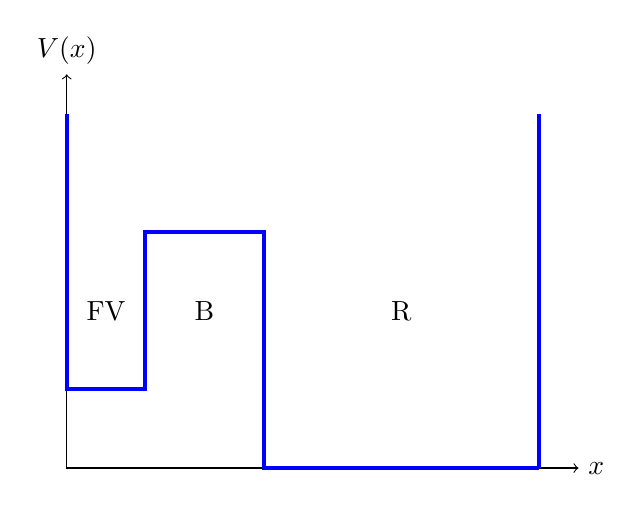
\begin{tikzpicture}
	
	\draw[<->] (6.5, 0) node[anchor = west] {$x$}-- (0,0) -- (0,5) node[anchor = south] {$V(x)$};
	
	\draw[blue, line width = 0.5mm] (0,0.975) -- (0, 4.5);
	\draw[blue, line width = 0.5mm] (-0.025,1) -- (1.025,1);
	\draw[blue, line width = 0.5mm] (1,0.975) -- (1,3.025);
	\draw[blue, line width = 0.5mm] (0.975,3) -- (2.5, 3);
	\draw[blue, line width = 0.5mm] (2.5, 3.025) -- (2.5,-0.025);
	\draw[blue, line width = 0.5mm] (2.475,0) -- (6,0);
	\draw[blue, line width = 0.5mm] (6,0) -- (6, 4.5);
	
	\node at (0.5, 2) (FV) {FV};
	\node at (1.75, 2) (B) {B};
	\node at (4.25, 2) (B) {R};
	
	\end{tikzpicture}
	\caption{Potencial para el estudio numérico del decaimiento del falso vacío. Cuenta con una región de falso (FV) y verdadero vacío (R), separados por una barrera (B) \cite{Masoumi:2015psa}.}
	\label{fig:potencial_numerico} 
\end{figure}

\begin{figure}[t]
	\centering
	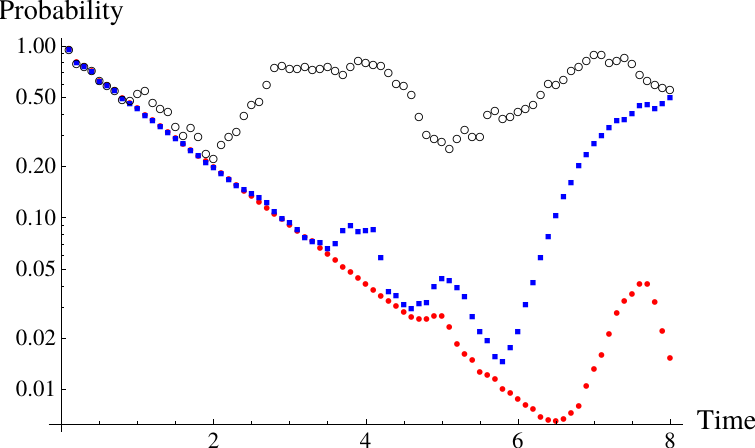
\includegraphics[scale = 0.4]{FIGURAS/numerico}
	\caption{Probabilidad de que una partícula permanezca en la región de falso vacío para distintos anchos de verdadero vacío. El eje vertical está en escala logarítmica \cite{Masoumi:2015psa}.}
	\label{fig:numerico}
\end{figure}

En la misma figura, sin embargo, puede apreciarse que el régimen lineal se mantiene solo durante un cierto intervalo de tiempo. Antes de atravesar la barrera, la función de onda oscila en la región del falso vacío,
%Esto se puede apreciar más fácilmente en la figura \ref{fig:numericoandreassen}. 
mientras que, cuando la función de onda ya atravesó la barrera y se encuentra la región del verdadero vacío, rebota con la pared infinita a la derecha y empieza a interactuar consigo misma, dando como resultado efectos no lineales \cite{Masoumi:2015psa}. Estos aspectos deben ser tomados en cuenta al momento de definir $\Gamma$ de manera precisa \cite{andreassen2017precision}. 

%\begin{figure}[h]
%	\centering
%	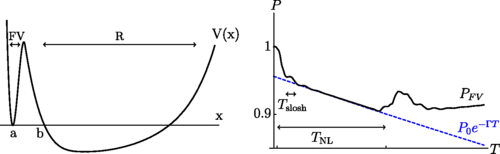
\includegraphics[scale = 0.7]{FIGURAS/numerico_andreassen}
%	\caption{\cite{andreassen2017precision}}
%	\label{fig:numericoandreassen}
%\end{figure}

%Siguiendo el formalismo de Coleman y Callan \cite{coleman1977fate, callan1977fate}, hallaremos una expresión para $\Gamma$ a primer orden en $\hbar$ . Puesto que el tunelamiento es un proceso no perturbativo, se hará uso de la integral de camino euclideana junto con la aproximación de punto estacionario.

%\colorbox{yellow}{añadir relacion entre WKB y falso vacio}

Haciendo uso de la aproximación WKB, es posible demostrar que $\Gamma$ es de la forma \cite{coleman1977fate}
\begin{equation} \label{eq:gamma_WKB}
\Gamma = Ae^{-B/\hbar}\qty(1 + \order{\hbar}),
\end{equation}
donde 
\begin{equation} \label{eq:B_WKB}
B = 2 \int_{x_+}^{p} \dd{x} \sqrt{2V\qty(x)}. 
\end{equation}

\section{Integral de camino euclideana}

%En el capítulo anterior pudimos determinar, analizando el tunelamiento usando la aproximación WKB, que el coeficiente $B$ en \eqref{eq:gamma} corresponde a la acción euclideana del bounce. Para calcular el coeficiente $A$ es necesario usar la integral de camino de Feynman en tiempo euclideano y la aproximación de punto estacionario. 

%El objetivo principal de este trabajo es calcular $\Gamma$ a primer orden en $\hbar$ para el estado metaestable de menor energía. Para esto se hará uso de la integral de camino euclideana y la aproximación de punto estacionario siguiendo principalmente el formalismo establecido por Coleman y Callan \cite{coleman1977fate, callan1977fate}. 

Consideremos una partícula que inicialmente se encuentra en la posición $x_i$ en un tiempo $t_i$. La amplitud de transición de esta a una posición final $x_f$ en un tiempo $t_f$ está dada por la integral de camino de Feynman \footnote{La integral de camino cuenta con una constante de normalización que debe ser elegida adecuadamente. Como no es de interés en este trabajo la asumiremos igual a 1.} \cite{feynman2010quantum}
\begin{equation}\label{eq:amplitud}
\bra{x_f, t_f}\ket{x_i, t_i} = \int \mathcal{D}x \, e^{iS\qty[x \qty(t)]/\hbar},
\end{equation}
donde $S\qty[x \qty(t)]$ es la acción de la partícula que, de la Mecánica Clásica, está dada por \footnote{A lo largo de todo el trabajo consideraremos que la partícula es de masa unitaria.}
\begin{equation}
S\qty[x \qty(t)] = \int \dd{t} \qty[\frac{1}{2} \left(\dv{x}{t}\right)^2 - V\qty(x)]. \label{eq:accion}
\end{equation}
%incluir explicacion de la integral de camino?

Una de las dificultades al momento de querer calcular \eqref{eq:amplitud} se debe al hecho de que está compuesta por una suma de fases complejas oscilatorias, que no necesariamente es convergente. Es por esto que resulta más conveniente trabajar en tiempo imaginario, para lo cual introducimos el tiempo euclideano $\tau$ mediante el cambio de variable
\begin{equation} \label{eq:tiempo_im}
	t = -i\tau, 
\end{equation} 
también conocido como rotación de Wick \cite{das2006field}. %Cabe mencionar que $\tau$ es un parámetro real. 

Aplicando \eqref{eq:tiempo_im} en la acción \eqref{eq:accion}, tenemos
\begin{align}
S\qty[x\qty(\tau)] &= \int \dd{\qty(-i\tau)} \qty[ \frac{1}{2} \left(\dv{x}{\qty(-i\tau)}\right)^2 - V(x)] \\
%&= -i\int \dd{\tau} \qty[ -\frac{1}{2} \left(\dv{x}{\tau}\right)^2 - V\qty(x)] \\ 
&= i \int \dd{\tau} \qty[ \frac{1}{2}\qty(\dv{x}{\tau})^2 + V(x)] \\
&= iS_E\qty[x\qty(\tau)] \label{eq:S_s_e}
\end{align}
donde hemos definido la acción euclideana $S_E\qty[x\qty(\tau)]$ como 
\begin{equation}\label{eq:eucliaction}
S_E\qty[x\qty(\tau)] \equiv \int \dd{\tau} \qty[ \frac{1}{2}\qty(\dv{x}{\tau})^2 + V(x)].
\end{equation}
%Haciendo de igual manera en la 
De igual manera, su ecuación de movimiento está dada por
%\begin{align}
%	\dv[2]{x}{t} &= -\dv{V(x)}{x} \\
%	\dv[2]{x}{\qty(-i\tau)} &= -\dv{V(x)}{x} \\
%	-\dv[2]{x}{\tau} &= -\dv{V(x)}{x},
%\end{align}
%obtenemos %la correspondiente para la acción euclideana, $S_E\qty[x\qty(\tau)]$,
\begin{equation}\label{eq:mov_ec}
\dv[2]{x}{\tau} = \dv{V(x)}{x},
\end{equation}
la cual puede ser interpretada como la ecuación de movimiento en tiempo real para una partícula moviéndose en el potencial invertido $-V\qty(x)$,
\begin{equation}
\dv[2]{x}{\tau} = -\dv{\qty(-V(x))}{x}.
\end{equation}
 
%Integrando la ecuación de movimiento \eqref{eq:mov_ec} respecto a la posición obtenemos la integral de movimiento
%\begin{align}
%	\dv[2]{x}{\tau} - \dv{V(x)}{x} &= 0 \\
%	\dv[2]{x}{\tau} - \dv{V(x)}{x} &= 0
%\end{align} 
Por último, en la energía, 
\begin{align}
	E &= \frac{1}{2} \left(\dv{x}{t}\right)^2 + V\qty(x) \\
%	&= \frac{1}{2} \left(\dv{x}{\qty(-i\tau)}\right)^2 + V\qty(x) \\
	&= -\frac{1}{2} \left(\dv{x}{\tau}\right)^2 + V\qty(x) \\
	&= -\mathcal{E}
\end{align}
donde hemos definido la energía euclideana $\mathcal{E}$ como \cite{rubakov2009classical}
\begin{equation} \label{eq:E_eucli}
	\mathcal{E}  \equiv \left(\dv{x}{\tau}\right)^2 - V\qty(x).
\end{equation}
%Como el potencial es independiente del tiempo, la energía euclideana se conserva. 

Al reemplazar \eqref{eq:S_s_e} en \eqref{eq:amplitud}, obtenemos la integral de camino euclideana \cite{das2006field}
\begin{equation}\label{eq:amplitud_euc}
I = \bra{x_f}e^{-HT/\hbar}\ket{x_i} = \int \mathcal{D}x \, e^{-S_E\qty[x\qty(\tau)]/\hbar},
\end{equation}
donde $T$ es el intervalo de tiempo euclideano que le toma a la partícula ir de $x_i$ a $x_f$. De esta manera, hemos convertido las fases oscilatorias en \eqref{eq:amplitud} en exponenciales decayentes que podremos calcular de manera aproximada mediante integrales gausianas, como se verá en la sección siguiente.

Insertamos una base de autoestados de energía $\qty{\ket{n}}$ en \eqref{eq:amplitud_euc} \cite{coleman1977fate}
\begin{equation}\label{eq:Eeigen}
I = \sum_n e^{-E_n T/\hbar} \bra{x_f}\ket{n}\bra{n}\ket{x_i}.
\end{equation}
%donde $\phi_n\qty(x) = \bra{x}\ket{n}$ es la función de onda del autoestado de energía $\ket{n}$. 
En el límite en el que $T \rightarrow \infty$, 
%que es en el que estamos interesados finalmente, 
la contribución de los términos de orden superior es exponencialmente pequeña, lo que nos permite extraer la energía del estado fundamental\footnote{Asumiendo que los autoestados de energía están normalizados.} \cite{andreassen2017precision}
\begin{equation} \label{eq:E_0}
	\frac{E_0}{\hbar} = -\lim_{T \rightarrow \infty} \frac{ \ln I}{T}.
\end{equation}

Como ya se discutió en la sección anterior,  %ver si de verdad se discutio
la energía del estado metaestable cuenta con una parte imaginaria, a partir de la cual obtenemos vacío $\Gamma$ a partir de la ecuación \eqref{eq:gammaE}. A su vez, $E_0$ está dado por \eqref{eq:E_0}, por lo que ahora podemos calcular $\Gamma$ directamente de la integral de camino euclideana \eqref{eq:amplitud_euc}
\begin{equation} \label{eq:Gamma}
	\Gamma = 2\Im\qty(\lim_{T \rightarrow \infty} \frac{ \ln I}{T}).
\end{equation}

\section{Aproximación de punto estacionario}

Los casos para los cuales es posible calcular la integral de camino de manera exacta son muy pocos y suelen involucrar técnicas matemáticas sofisticadas \cite{feynman2010quantum, das2006field, kleinert2009path}, por lo que usualmente se tiene que recurrir a métodos aproximados. En nuestro caso, haremos uso de la aproximación de punto estacionario (\emph{saddle point approximation} 
%\footnote{En este trabajo, punto estacionario y punto de silla son sinónimos.}
) para calcular la integral de camino euclideana en \eqref{eq:Gamma}. 

Al igual que en el cálculo diferencial, los puntos estacionarios de la acción euclideana $S_E\qty[x\qty(\tau)]$ son aquellos que cumplen con la condición
\begin{equation}\label{eq:minimo}
	\fdv{S_E\qty[x\qty(\tau)]}{x\qty(\tau)} = 0.
\end{equation}
Esto no es más que el principio de mínima acción de la Mecánica Clásica, por lo que los puntos estacionarios corresponden a las trayectorias clásicas $x_{\text{cl}}\qty(\tau)$, soluciones de la ecuación de movimiento \eqref{eq:mov_ec}. Por simplicidad, supondremos que tenemos un único punto estacionario.

Expandiendo $S_E\qty[x\qty(\tau)]$ alrededor de la trayectoria clásica $x_{\text{cl}}\qty(\tau)$,
\begin{equation} \label{eq:trayec}
	x\qty(\tau) = x_{\textrm{cl}}\qty(\tau) + \eta\qty(\tau),
\end{equation}
donde $\eta\qty(\tau)$ es la variación respecto a la trayectoria clásica sujeta a las condiciones de frontera
\begin{equation}
	\eta\qty(\tau_i) = \eta\qty(\tau_f) = 0,
\end{equation}
tenemos,
\begin{align} 
S_{E}\qty[x\qty(\tau)] &= S_{E}[x_{\textrm{cl}}(\tau) +  \eta\qty(\tau)] \\ 
&= S_{E}[x_{\textrm{cl}}\qty(\tau)]
%+ \int \dd{\tau_1}\eta(\tau_1) 	\fdv{S_E\qty[x_{\textrm{cl}}\qty(\tau_1)]}{x_{\textrm{cl}}\qty(\tau_1)} 
+ \frac{1}{2} \int \dd{\tau_1} \dd{\tau_2} \eta(\tau_1) \frac{\delta^2 S_E[x_{\textrm{cl}}\qty(\tau)]}{\var{x_{\textrm{cl}}\qty(\tau_1)} \var{x_{\textrm{cl}}\qty(\tau_2)}} \eta\qty(\tau_2) + \order{\eta^3}. \label{eq:approx1}
\end{align}
El primer término corresponde a la acción euclideana clásica  $S_E^{\textrm{cl}}$. Por conveniencia, definimos la variación de segundo orden como
\begin{equation}
	S_E^{(2)} \equiv \frac{1}{2} \int \dd{\tau_1} \dd{\tau_2} \eta\qty(\tau_1) \frac{\delta^2 S_E[x_{\textrm{cl}}\qty(\tau)]}{\var{x_{\textrm{cl}}(\tau_1)} \var{x_{\textrm{cl}}\qty(\tau_2)}} \eta\qty(\tau_2). \label{eq:S_2}
\end{equation}
El término lineal se cancela  por \eqref{eq:minimo}.%, debido a que la trayectoria clásica es un punto estacionario de la acción. 

En comparación con los términos anteriores, el valor de $\hbar$ es pequeño. Esto nos permite ignorar los términos de orden superior en \eqref{eq:approx1}. Para verlo más claramente, reemplacemos $S_{E}\qty[x\qty(\tau)]$ en \eqref{eq:amplitud_euc} por \eqref{eq:approx1},
\begin{equation}\label{eq:Iaprox1}
I = e^{-S_E^{\textrm{cl}}/\hbar} \int \mathcal{D}\eta \, e^{-S_E^{(2)}/\hbar + \order{\eta^3}},
\end{equation}
donde, al haber fijado el camino clásico, ahora integramos sobre todas sus variaciones, cambiando la medida de integración. Reescalando $\eta\qty(\tau) \rightarrow \sqrt{\hbar}\eta\qty(\tau)$ \footnote{La nueva medida de integración incluye un factor constante que absorbemos en $N$.},
\begin{equation}\label{eq:Iaprox2}
I = e^{-S_E^{\textrm{cl}}/\hbar} \int \mathcal{D}\eta \, e^{-S_E^{(2)} + \order{\hbar}}
\end{equation}
notamos que los términos de orden superior en \eqref{eq:approx1} son de primer orden en $\hbar$, justificando la aproximación \cite{paranjape2017theory}. Esta es la razón por lo que la aproximación de punto estacionario es un método semiclásico. Será a este orden que calcularemos la tasa de decaimiento del falso vacío $\Gamma$. 

La derivada funcional de la acción euclideana \eqref{eq:eucliaction} es igual a la ecuación de movimiento \eqref{eq:mov_ec}
\begin{equation} \label{eq:dev1}
	\fdv{S_E\qty[x\qty(\tau)]}{x\qty(\tau_1)} = -\ddot{x}\qty(\tau_1) + V'\qty(\tau_1),
\end{equation}
donde el punto indica la derivada respecto a $\tau$, mientras que la prima indica la derivada respecto a $x\qty(\tau)$. Tomando la derivada funcional de \eqref{eq:dev1} y desarrollando 
\begin{align}
\frac{\var{S_E[x\qty(\tau)]}}{{\var{x}(\tau_1)} \var{x}\qty(\tau_2)} &= -\fdv{\ddot{x}\qty(\tau_1)}{x\qty(\tau_2)} + \fdv{V'\qty(x)}{x\qty(\tau_2)} \\
&= -\dv[2]{\tau_1}\qty(\fdv{x\qty(\tau_1)}{x\qty(\tau_2)}) + V''\qty(x)\fdv{x\qty(\tau_1)}{x\qty(\tau_2)} \\
&= \qty(-\dv[2]{\tau_1} + V''\qty(x)) \delta\qty(\tau_1 - \tau_2).
\end{align}
Reemplazando en \eqref{eq:S_2},
\begin{align}
	S_E^{(2)} &= \frac{1}{2} \int \dd{\tau_1} \dd{\tau_2} \eta\qty(\tau_1) \qty(-\dv[2]{\tau_1} + V''\qty(x_{\text{cl}}))\delta\qty(\tau_1 - \tau_2) \eta\qty(\tau) \\ \label{eq:S_2_1}
	&= \frac{1}{2} \int \dd{\tau} \eta\qty(\tau) \qty(-\dv[2]{\tau} + V''\qty(x_{\text{cl}})) \eta\qty(\tau),
\end{align}
notamos que el cálculo de $S_E^{(2)}$ está íntimamente relacionado con el operador
\begin{equation} \label{eq:operador}
	\hat{O} \equiv -\dv[2]{\tau} + V''\qty(x_{\text{cl}}).
\end{equation}

Introduzcamos una base de autofunciones del operador anterior $\qty{\eta_i \qty(\tau)}$ \cite{rubakov2009classical}
\begin{equation} \label{eq:eigen1}
\qty( - \dv[2]{\tau} + V''\qty(x_{\text{cl}})) \eta_\lambda\qty(\tau) = \lambda \eta_\lambda\qty(\tau),
\end{equation}
tal que podemos expandir $\eta\qty(\tau)$ en función de esta
 \begin{equation}\label{eq:eigen3}
\eta\qty(\tau) = \sum_\lambda c_\lambda \eta_\lambda \qty(\tau). 
\end{equation}
Como la base es completa y ortonormal, 
\begin{equation} \label{eq:eigen2}
\int \dd{\tau} \eta_{\lambda'}\qty(\tau) \eta_{\lambda}\qty(\tau) = \delta_{\lambda'\lambda}.
\end{equation}
Insertando \eqref{eq:eigen3} en \eqref{eq:S_2_1} y usando \eqref{eq:eigen1} y \eqref{eq:eigen2},
\begin{align}
S_E^{(2)} &= \frac{1}{2} \int \dd{\tau}\qty( \sum_{\lambda'} c_{\lambda'} \eta_{\lambda'} \qty(\tau)) \qty(-\dv[2]{\tau} + V''\qty(x_{\text{cl}})) \qty( \sum_\lambda c_\lambda \eta_\lambda \qty(\tau)) \\
&= \frac{1}{2} \sum_{\lambda'} \sum_\lambda \lambda c_\lambda' c_\lambda \int \dd{\tau} \eta_\lambda' \qty(\tau)  \eta_\lambda \qty(\tau) \\
&= \frac{1}{2} \sum_{\lambda'} \sum_\lambda \lambda c_\lambda' c_\lambda \delta_{\lambda'\lambda} \\
&= \frac{1}{2} \sum_\lambda \lambda c_\lambda^2. \label{eq:S_2_2}
\end{align}

Al momento de reemplazar \eqref{eq:S_2_2} en \eqref{eq:Iaprox1}, pasamos a integrar sobre todos los coeficientes $\qty{c_\lambda}$, por lo que elegimos como medida de integración 
\begin{equation}
	\mathcal{D}\eta = \prod_\lambda \frac{\dd{c_\lambda}}{\sqrt{2\pi \hbar}},
\end{equation}
donde incluimos los factores $\sqrt{2\pi \hbar}$ por conveniencia. 
%Estos solo afectan a la constante de normalización $N$. 
Tomando todo esto en cuenta, \eqref{eq:Iaprox1} se reduce a un producto de integrales gausianas cuyo resultado es conocido y fácil de calcular
\begin{align} 
I &\approx e^{-S_E^{\textrm{cl}}/\hbar} \int \prod_\lambda \frac{\dd{c_\lambda}}{\sqrt{2\pi \hbar}} e^{-\sum_\lambda \lambda c_\lambda^2/2\hbar} \\
&= e^{-S_E^{\textrm{cl}}/\hbar} \prod_\lambda \int  \frac{\dd{c_\lambda}}{\sqrt{2\pi \hbar}} e^{-\lambda c_\lambda^2/2\hbar} \\ \label{eq:I_gauss}
&= e^{-S_E^{\textrm{cl}}/\hbar} \prod_\lambda \lambda^{ -1/2}.
\end{align}
%\begin{equation} 
%I 
%&\approx N e^{-S_E^{\textrm{cl}}/\hbar} \int \prod_\lambda \frac{\dd{c_\lambda}}{\sqrt{2\pi \hbar}} \prod_\lambda e^{-\lambda c_\lambda^2/2\hbar} \\ 
%\end{equation}

El producto de los autovalores en el último término de \eqref{eq:I_gauss} no es más que la determinante de $\hat{O}$. Con esto, %tenemos finalmente que 
la amplitud de transición en la aproximación de punto estacionario está dada por
\begin{equation}\label{eq:Isaddle}
I = e^{-S_E^{\textrm{cl}} / \hbar} \qty[ \det\left(-\dv[2]{\tau} + V''\qty(x_{\textrm{cl}}) \right) ]^{-1/2} \qty(1 + \order{\hbar}).
\end{equation}
Cabe resaltar que esta aproximación es de primer orden en $\hbar$. En caso la acción euclideana posea múltiples puntos estacionarios, debemos sumar la contribución de cada uno.

%Notamos que la amplitud consta de un término no perturbativo dado por la exponencial y 

En la derivación anterior hemos supuesto implícitamente que todos los autovalores de $\hat{O}$ son positivos. De no ser así, \eqref{eq:Isaddle} falla y tendríamos que tratar por separado aquellos autovalores que no cumplan con está condición, resultando en factores adicionales. %en la ecuación \eqref{eq:Isaddle}. 
Como veremos en las secciones siguientes, este es el caso para el decaimiento del falso vacío.

\section{Bounce}

%Para calcular la integral de camino euclideana \eqref{eq:Isaddle} Los puntos estacionarios correspondientes al decaimiento del falso vacío corresponden a las trayectorias clásicas de una partícula movi para un potencial como el de la figura \ref{fig:potencial}. 

 
%Al momento de calcular $\Gamma$ usando la ecuación \eqref{eq:Gamma} estamos interesados en el límite cuando $T$ se hace infinito.  
%Usando la ecuación la tasa de decaimiento del falso vacío $\Gamma$ 
%Para poder calcular la amplitud $I$ dada por la ecuación \eqref{eq:Isaddle} en el caso del decaimiento del falso vacío, debemos hallar las trayectorias clásica correspondientes, al ser los puntos estacionarios de la acción euclideana $S_E\qty[x\qty(\tau)]$,
%Como se discutió en la sección inicial de este capítulo, obtendremos la tasa de decaimiento del falso vacío $\Gamma$ a partir de la amplitud $I$ correspondiente. Para esto haremos uso de la ecuación \eqref{eq:Isaddle}, pero antes necesitamos conocer las trayectorias clásicas 

Como se discutió en la sección inicial de este capítulo, la tasa de decaimiento del falso vacío está relacionada con la probabilidad de que una partícula permanezca en la región del falso vacío del potencial. %como los de las figuras \ref{fig:potencial} y \ref{fig:potencial_numerico}. 
Es por esto que las trayectorias clásicas, necesarias para calcular la amplitud de transición en la aproximación de punto estacionario usando la ecuación \eqref{eq:Isaddle}, deben empezar y terminar en dicha región. Es decir, $x_i = x_f = x_+$. 
%Al momento de realizar la aproximación de punto estacionario, consideramos que la partícula va de la posición inicial a la final en un intervalo de tiempo euclideano $T$ finito. Sin embargo, %puesto que obtendremos $\Gamma$ a partir de la ecuación \eqref{eq:Gamma}, 
%estamos interesados en el límite $T \rightarrow \infty$ 
%Además, estamos interesados en el límite en el que el intervalo de tiem po euclideano $T$ se hace infinito \cite{coleman1977fate}. 
%
%tomando como referencia la figura \ref{fig:potencial}. 

Las trayectorias clásicas deben ser entonces las soluciones de la ecuación de movimiento \eqref{eq:mov_ec} con las condiciones de frontera \cite{coleman1977fate}
\begin{equation} \label{eq:cond_frontera}
	\lim_{\tau \rightarrow \pm\infty} x\qty(\tau) = x_+.
\end{equation} 
Las trayectorias clásicas obtenidas no serán las exactas, pero son buenas aproximaciones, especialmente a medida que tomamos intervalos de tiempo euclideano cada vez mayores, que es el límite en el que estamos interesados finalmente \cite{paranjape2017theory, callan1977fate}. Por conveniencia, tomaremos $\tau_i = -T/2$ y $\tau_f = T/2$, tal que cuando necesitemos considerar el intervalo de tiempo euclideano finito este sea igual a $T$. 
%donde hemos considerado el hecho de que Si bien las trayectorias que obtendremos no son exactamente los puntos estacionarios, representan buenas aproximaciones especialmente a medida que hacemos $T$ cada vez mayor. 

\begin{figure}[t]
	\centering
	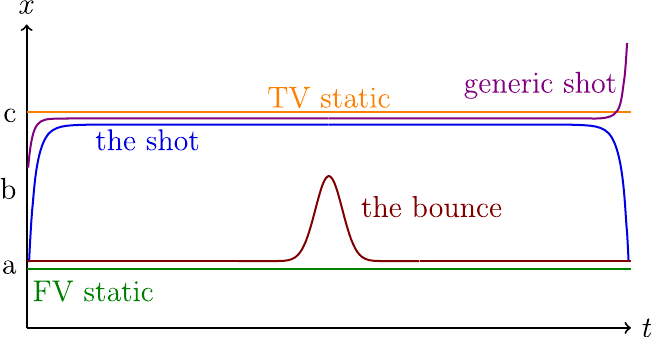
\includegraphics[scale=0.375]{FIGURAS/soluciones}
	\caption{Trayectorias clásicas para el decaimiento del falso vacío \cite{andreassen2017precision}. 
		%Los puntos $a$, $b$ y $c$ corresponden a $x_-$, $p$ y $x_+$ respectivamente .
	}
	\label{fig:soluciones}
\end{figure}

En la figura \ref{fig:soluciones} se encuentran ilustradas las trayectorias clásicas a considerar. La primera es la solución trivial $x_{\text{FV}}\qty(\tau)$ (\emph{FV static} en la figura \ref{fig:soluciones}) en la que la partícula permanece en el falso vacío para todo $\tau$,
\begin{equation}
x_{\text{FV}}\qty(\tau) = x_+.
\end{equation} 
Como $V\qty(x_+) = 0$ y la solución es constante, $S_E[x_{\text{FV}}\qty(\tau)] = 0$ 
y su contribución a la amplitud de transición $I_0$ es simplemente %\footnote{Omitimos la constante de normalización puesto que no es de interés.}
\begin{equation}
	I_0 = \qty[ \det\left(-\dv[2]{\tau} + \omega^2 \right) ]^{-1/2},
\end{equation}
donde hemos definido %la frecuencia de oscilación alrededor de $x_+$ $\omega$ como
\begin{equation}
	\omega^2 \equiv V''\qty(x_+).
\end{equation}
%El subíndice hace referencia a que es la contribución de la solución estática. 
%Si bien es posible calcular la determinante \cite{das2006field}, no será necesario. %la frecuencia de oscilación alrededor de $x_+$ 
De igual manera, %$\mathcal{E} = 0$.
su energía euclideana también es nula. %Requeriremos que esta condición se cumpla para el resto de trayectorias clásicas.

%Notamos rápidamente que tenemos una primera trayectoria clásica en la que la partícula permanece en el falso vacío todo el tiempo. Llamaremos a esta solución  
%es la solución trivial de \eqref{eq:mov_ec} que cumple  \eqref{eq:cond_frontera}.

Analizando el potencial invertido de la figura \ref{fig:potencial_invertido} notamos que es posible encontrar trayectorias clásicas no triviales que atraviesen la barrera del potencial original. Consideremos una partícula que inicia su movimiento en $x_+$. Como el potencial es plano alrededor de este punto, permanece ahí por un largo tiempo, para luego recorrer rápidamente el pozo de potencial invertido hasta llegar al punto de retorno $p$ en un tiempo finito. %0y regresa nuevamente a $x_+$. 
La invarianza de la acción euclideana ante inversiones temporales  nos permite extender esta trayectoria de vuelta a $x_+$ \cite{weinberg2012classical}. Si $\tau_i = -\infty$ y $\tau_f = +\infty$,
%los tiempos euclideanos inicial y final son $\tau = \pm \infty$ respectivamente
obtenemos el bounce \footnote{Mantendremos el nombre en l idioma original por ser el término comúnmente usado en la literatura.}  $x_B\qty(\tau)$ \cite{coleman1977fate}. Su comportamiento se encuentra ilustrado en las figuras \ref{fig:soluciones} y \ref{fig:bounce}. 
%Al igual que para la solución estática, su energía euclideana también es nula. 

\begin{figure}[h]
	\centering
	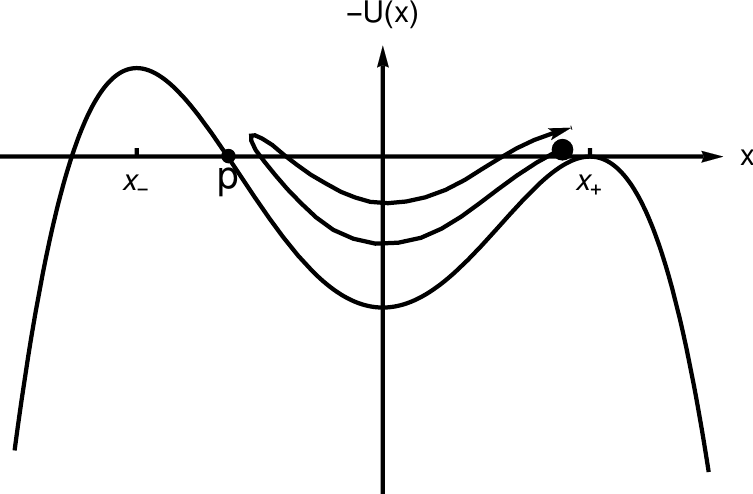
\includegraphics[scale = 0.3]{FIGURAS/potencial_invertido}
	\caption{Potencial invertido  correspondiente al de la figura \ref{fig:potencial} \cite{Ai:2019dqr}.}
	\label{fig:potencial_invertido}
\end{figure}
%Esta solución es de tipo instanton y su existencia esta garantizada por la invarianza de la acción euclideana ante inversiones temporales \cite{paranjape2017theory, weinberg2012classical}.

%Para describir el bounce, tenemos que tomar en cuenta que su energía euclideana debe ser nula. La partícula parte lentamente de $x_+$, donde permanece durante un largo tiempo puesto que el potencial es plano alrededor de este punto. Luego,    Este comportamiento se ilustra en las figuras \ref{fig:soluciones} y \ref{fig:bounce}.


\begin{figure}[t]
	\centering
	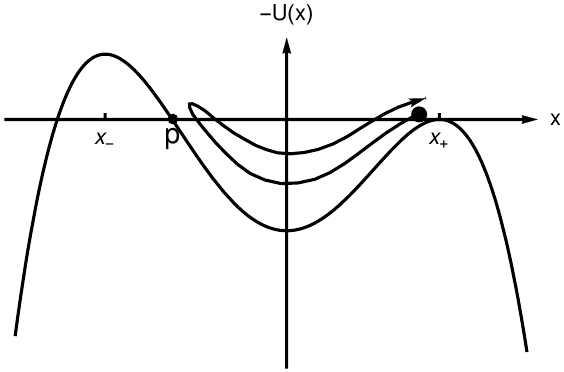
\includegraphics[scale=0.25]{FIGURAS/bounce}
	\caption{Bounce \cite{weinberg2012classical}. %El punto $b$ corresponde al punto de retorno $p$.
	}
	\label{fig:bounce}
\end{figure}

%Para calcular su acción euclideana, partimos del hecho de que la 
Aprovechando el hecho de que el bounce es invariante ante translaciones temporales, posicionemos su centro, correspondiente al instante en el que la partícula llega a $p$ , en $\tau = 0$ \cite{coleman1977fate}. La partícula se detiene en ese punto, por lo que
\begin{equation} \label{eq:vel}
\eval{\dv{x_B}{\tau}}_{\tau = 0} = 0.
\end{equation}
%Esta condición tendrá implicaciones importantes más adelante. 
Como $V\qty(p) = 0$, la energía euclideana del bounce también es nula debido al principio de conservación de la energía. De la definición en \eqref{eq:E_eucli}, tenemos que
\begin{equation} \label{eq:K=V}
\frac{1}{2}\qty(\dv{x_B}{\tau})^2 = V\qty(x_B).
\end{equation}

La acción euclideana del bounce está dada por %\footnote{La elección de notación se hará evidente al finalizar el cálculo.} 
\begin{equation}\label{eq:S_B1}
S_E\qty[x_B\qty(\tau)] =  \int_{-\infty}^{+\infty} \dd{\tau} \qty[ \frac{1}{2}\qty(\dv{x_B}{\tau})^2 + V\qty(x_B) ]. 
\end{equation}
Si dividimos la integral en $\tau = 0$,
\begin{equation}\label{eq:S_B_tau0}
S_E\qty[x_B\qty(\tau)] =  \int_{-\infty}^{0} \dd{\tau} \qty[ \frac{1}{2}\qty(\dv{x_B}{\tau})^2 + V\qty(x_B) ] +   \int_{0}^{+\infty} \dd{\tau} \qty[ \frac{1}{2}\qty(\dv{x_B}{\tau})^2 + V\qty(x_B) ]. 
\end{equation}
y hacemos $\tau \rightarrow -\tau$ en la segunda integral, ambos términos son iguales. %, tal que 
%Como el bounce es simétrico, ambas integrales son iguales %su acción euclideana es el doble del recorrido de ida es igual al del de retorno %es suficiente con solo considerar la parte de la trayectoria que va de $x_+$ a $p$.  
%\begin{equation}\label{eq:S_B2}
%S_E\qty[x_B\qty(\tau)] =  2\int_{-\infty}^{0} \dd{\tau} \qty[ \frac{1}{2}\qty(\dv{x_B}{\tau})^2 + V\qty(x_B) ].
%\end{equation}
Esto es una consecuencia directa de la invariancia de la acción euclideana ante inversiones temporales, relacionada también con la simetría del bounce. Si además usamos \eqref{eq:K=V}, podemos reducir \eqref{eq:S_B1} a
\begin{equation} \label{eq:S_B3}
S_E\qty[x_B\qty(\tau)] = 2\int_{-\infty}^{0} \dd{\tau} 2 V\qty(x_B).
\end{equation}
%Dividamos la integral en $\tau = 0$ 
%\begin{equation}\label{eq:S_B4}
%B =  \int_{-\infty}^{0} \dd{\tau} 2 V\qty(x_B) + \int_{0}^{+\infty}   \dd{\tau} 2 V\qty(x_B)
%\end{equation}
Por último, realicemos el cambio variable $\tau \rightarrow x_B$ \cite{rubakov2009classical}. Despejando $\text{d}x_B/\text{d}\tau$ en \eqref{eq:K=V}, %obtenemos $\dd{\tau}$ en función de $\dd{x_B}$, 
\begin{align}
\dv{x_B}{\tau} &= \sqrt{2V\qty(x_B)} \\  \label{eq:dtau}
\dd{\tau} &= \frac{\dd{x_B}}{\sqrt{2V(x_B)}}.
\end{align}
%Los nuevos límites de integración son a su vez,  
Reemplazando \eqref{eq:dtau} en \eqref{eq:S_B3} con los límites de integración correspondientes,
\begin{equation}
x_B\qty(-\infty) = x_+, \quad x_B\qty(0) = p,
\end{equation}
obtenemos finalmente
\begin{equation}\label{eq:bounce4}
S_E\qty[x_B\qty(\tau)] = 2 \int_{x_+}^{p} \dd{x} \sqrt{2 V\qty(x)},
\end{equation}
donde hemos omitido el subíndice al ya no ser necesario. Notamos que la acción euclideana del bounce es igual al coeficiente $B$ en la ecuación \eqref{eq:B_WKB}, 
\begin{equation}
	B = S_E\qty[x_B\qty(\tau)].
\end{equation}
%La conexión entre la aproximación WKB y la aproximación de punto estacionario se explorará en mayor detalle al considerar el tunelamiento en varias dimensiones. 

%\colorbox{yellow}{mejorar redaccion}
 
%A diferencia de lo que tuvimos con la solución trivial, 
Al momento de calcular la contribución del bounce a la amplitud de transición, no podemos hacer uso de \eqref{eq:Isaddle} directamente debido a que, en este caso, $\hat{O}$ cuenta con autovalores que no son positivos. En las secciones a continuación, se discutirán las complicaciones que esto conlleva y cómo solucionarlas. 
%En las secciones a continuación exploraremos dichas dificultades y como resolverlas. %que el cero es un autovalor de $\hat{A}$ y además posee uno negativo. Este último es el que contribuirá con la parte imaginaria de la energía necesaria para obtener $\Gamma$. \colorbox{yellow}{mejorar redaccion}

\subsection{Modo cero} \label{sec:modo_zero}

Por construcción, el bounce es una solución de la ecuación de movimiento \eqref{eq:mov_ec},
\begin{equation}\label{eq:mov_ec_bounce}
\dv[2]{x_B}{\tau} - V' \qty(x_B) = 0.
\end{equation}
Al derivar la ecuación anterior respecto a $\tau$,
\begin{align}
	\dv{\tau}\qty(\dv[2]{x_B}{\tau} - V'\qty(x_B)) &= 0 \\
	\dv[2]{\tau}\qty(\dv{x_B}{\tau}) - V''\qty(x_B)\dv{x_B}{\tau} &= 0 \\
	\qty(\dv[2]{\tau} - V''\qty(x_B))\dv{x_B}{\tau} &= 0, \label{eq:eom_modo_cero}
\end{align}
se muestra claramente que $\hat{O}$ cuenta con un autovector cuyo autovalor es igual a cero. Por esta razón decimos que $\hat{O}$ cuenta con un modo cero.
%y de hecho, este siempre es el caso .

%Normalicemos $\text{d}x_B/\text{d}\tau$. 
Los autovalores de $\hat{O}$ deben estar están normalizados. De \eqref{eq:S_B1} y usando \eqref{eq:K=V}, tenemos que
\begin{equation}
	\int_{-\infty}^{+\infty} \dd{\tau} \qty(\dv{x_B}{\tau})^2 = B,
\end{equation}
de tal manera que el modo cero $x_0\qty(\tau)$, proporcional a $\text{d}x_B/\text{d}\tau$, está dado por %\footnote{En \cite{callan1977fate} se denomina al modo cero como $x_1\qty(\tau)$.}
\begin{equation}
	x_0(\tau) = B^{-1/2} \dv{x_B}{\tau}.
\end{equation}

Como ya se ha comentado anteriormente, el modo cero representa un problema al momento de calcular la contribución del bounce a la amplitud de transición. Para verlo explícitamente, retornemos a la ecuación \eqref{eq:I_gauss}, en la que expresamos la amplitud de transición como un producto de integrales gausianas, y separemos la integral respecto al coeficiente $c_0$ correspondiente al modo cero, 
\begin{equation} \label{eq:integral_0}
	\int \frac{\dd{c_0}}{\sqrt{2\pi \hbar}} 
	%\prod_{\lambda \neq 0} \int  \frac{\dd{c_\lambda}}{\sqrt{2\pi \hbar}} e^{-\lambda c_\lambda^2/2\hbar}.
\end{equation}
Puesto que $\lambda = 0$, hemos perdido el amortiguamiento exponencial relacionado con $c_0$ por lo que \eqref{eq:integral_0}
% la integral resultante
, es divergente. 

La existencia de un modo cero está siempre relacionada con una simetría del sistema \cite{das2006field}. 
%Siempre que se presenta un modo cero, está relacionado con alguna simetría de la acción. 
En este caso, es debido a la simetría de la acción euclideana ante traslaciones temporales \cite{callan1977fate}. Si bien, por conveniencia, fijamos el centro del bounce en $\tau = 0$, bien podríamos haberlo hecho en cualquier otro instante de tiempo euclideano. Esto significa que existe un conjunto de bounces, cuyos centros están localizados a lo largo de todo el intervalo de tiempo euclideano, que también son soluciones de la ecuación de movimiento y por lo tanto, también contribuyen a la amplitud de transición. Este es el origen de la divergencia 
%de la integral en \eqref{eq:integral_0} 
\cite{kleinert2009path}.

Analíticamente, una traslación temporal es equivalente a realizar la siguiente transformación,
\begin{equation}
x_B \qty(\tau - \tau_0) = e^{-\tau_0 \dv{\tau}} x_B \qty(\tau).
\end{equation}
Al efectuar esta transformación, desplazamos al bounce de tal manera que su centro se encuentra ahora en $\tau_0$.
%Podemos realizar  por 
%%desplazamos el centro del bounce  mediante la transformación
%\begin{equation}
%	x_B \qty(\tau - \tau_0) = e^{-\tau_0 \dv{\tau}} x_B \qty(\tau),
%\end{equation}
%desplazamos su centro obteniendo un nuevo bounce cuyo centro se encuentra ahora en $\tau_0$. 
Como se discutió anteriormente, $x_B \qty(\tau - \tau_0)$ también es solución de la ecuación de movimiento \eqref{eq:mov_ec},
\begin{equation} \label{eq:eom_bounce1}
\dv[2]{\tau}x_B \qty(\tau - \tau_0) - V'(x_B \qty(\tau - \tau_0)) = 0. 
\end{equation}

Consideremos una transformación infinitesimal,
\begin{equation} \label{eq:bounce_inf}
x_B \qty(\tau - \var{\tau_0}) \approx x_B \qty(\tau) -  \dv{x_B }{\tau}\var{\tau_0},
\end{equation}
en \eqref{eq:eom_bounce1},
\begin{equation}
\dv[2]{\tau} \qty(x_B \qty(\tau) -  \dv{x_B}{\tau}\var{\tau_0}) - V'\qty(x_B \qty(\tau) - \dv{x_B}{\tau}\var{\tau_0}) = 0.
\end{equation}
Expandiendo el segundo término a primer orden en $\tau_0$ y reordenando,
\begin{equation}
\qty(\dv[2]{x_B \qty(\tau)}{\tau} - V'\qty(x_B)) -  \qty(\dv[2]{\tau} - V''\qty(x_B))\dv{x_B}{\tau}\var{\tau_0} = 0.
\end{equation}
El primer término se anula debido a que el bounce es solución de la ecuación de movimiento, por lo que obtenemos nuevamente el resultado en la ecuación \eqref{eq:eom_modo_cero}, 
\begin{equation}
\qty(\dv[2]{\tau} - V''\qty(x_B))\dv{x_B}{\tau} = 0.
\end{equation}
Con esto, hemos demostrado la existencia del modo cero a partir de la simetría del sistema ante traslaciones temporales. 

Veamos ahora cómo solucionar el problema de la divergencia en el cálculo de la contribución del bounce a la amplitud de transición. 
%Para solucionar el problema al calcular \eqref{eq:integral_0}, reemplazaremos $c_0$ por una coordenada colectiva relacionada con la simetría, es decir, $\tau_0$. %método conocido como coordenada colectiva. 
Para esto es necesario reemplazar $c_0$
%el coeficiente  correspondiente al modo cero 
por una coordenada colectiva relacionada con la simetría correspondiente del sistema . En nuestro caso, debemos hacer uso de $\tau_0$  %que especifica la ubicación del centro del bounce 
\cite{weinberg2012classical, paranjape2017theory}. 
%Como $x_B \qty(\tau - \tau_0)$ es una trayectoria clásica, podemos expandir cualquier otra trayectoria alrededor de esta,

Consideremos la expansión de la trayectoria $x\qty(\tau)$ alrededor del bounce
\begin{equation} \label{eq:trayec_bounce}
x\qty(\tau) 
%&= x_{B}\qty(\tau) + \eta\qty(\tau) \\
%&= x_B \qty(\tau) + c_0\eta\qty(\tau) + \sum_{\lambda \neq 0} c_\lambda\eta_\lambda\qty(\tau) \\
= x_B \qty(\tau) + c_0 B^{-1/2} \dv{x_B}{\tau} + \sum_{\lambda \neq 0} c_\lambda\eta_\lambda\qty(\tau).
\end{equation}
%Para introducir $\tau_0$ , Hacemos de igual manera, pero alrededor de  
%\begin{equation} \label{eq:trayec_bounce_t0}
%x\qty(\tau) = x_B \qty(\tau - \tau_0) + \xi\qty(\tau - \tau_0).
%\end{equation}
%Al realizar un cambio infinitesimal en $c_0$, este tiene como resultado
La variación de la trayectoria debido a un cambio infinitesimal en $c_0$ está dado por
\begin{equation} \label{eq:modo0_aprox1}
	B^{-1/2} \dv{x_B}{\tau} \var{c_0}.
\end{equation}
Comparando \eqref{eq:modo0_aprox1} con \eqref{eq:bounce_inf}, notamos que el primero es equivalente a la variación de la trayectoria debido a un desplazamiento infinitesimal del centro del bounce $\var{\tau_0}$ igual a \begin{equation} \label{eq:var_tau}
	\var{\tau_0} = -B^{-1/2} \var{c_0}.
\end{equation} 
%De igual manera, si expandimos $S_E\qty[x\qty(x)]$ alrededor de $x_B \qty(\tau - \tau_0)$ y , la variación de la trayectoria debido a un cambio en $\tau_0$ está dada por
%\begin{equation} \label{eq:modo0_aprox 2}
%\dv{x_B}{\tau} \dd{\tau_0}.
%\end{equation}
%Comparando \eqref{eq:modo0_aprox 1} y \eqref{eq:modo0_aprox 2}, 
%de donde obtenemos directamente que el jacobiano, a primer orden en $\hbar$, para el 
Tenemos entonces que, al realizar el cambio de variable de $c_0$ a $\tau_0$ a primer orden en $\hbar$, la contribución del bounce a la amplitud de transición $I_1$  adquiere un factor adicional de $ B^{1/2}$ \footnote{Una derivación detallada de este resultado requiere el uso del truco de Faddeev-Popov \cite{kleinert2009path, rubakov2009classical, andreassen2017precision}.} \cite{das2006field, kleinert2009path}.
%\begin{equation} \label{eq:jacobiano}%
%	\qty|\dv{c_0}{\tau_0}| = B^{1/2}.
%\end{equation}
%Si bien $\tau_0$ también debe ir de $+\infty$ a $-\infty$

Con esto, e integrando sobre el intervalo de tiempo euclideano finito $\tau_0 \in \qty[-T/2, T/2]$, %la contribución del bounce a la amplitud de transición está dada por
\begin{align}
	I_1 &= e^{-B/\hbar} \int_{-T/2}^{T/2} \dd{\tau_0}\qty(\frac{B}{2\pi \hbar})^{1/2} \prod_{\lambda \neq 0} \int  \frac{\dd{c_\lambda}}{\sqrt{2\pi \hbar}} e^{-\lambda c_\lambda^2/2\hbar}  \\
	%&= N\qty(\frac{B}{2\pi \hbar})^{1/2} \qty[ \text{det}'\left(-\dv[2]{\tau} + V''\qty(x_B) \right) ]^{-1/2} Te^{-B/\hbar}
	&= T\qty(\frac{B}{2\pi \hbar})^{1/2} e^{-B/\hbar}  \prod_{\lambda \neq 0} \int \frac{\dd{c_\lambda}}{\sqrt{2\pi \hbar}} e^{-\lambda c_\lambda^2/2\hbar},
\end{align}
%donde la prima en la determinante significa que solo consideramos los autovalores positivos. Incluimos el subíndice para indicar que corresponde a la contribución de un único bounce. 
hemos resuelto el problema de la divergencia relacionada a la existencia del modo cero. Sin embargo, aún no podemos terminar con el cálculo debido a que existe otra fuente de divergencia aún más grave: $\hat{O}$ cuenta con un autovalor negativo en su espectro, el cual se discutirá en la sección a continuación.  

\subsection{Modo negativo} 

Al analizar la forma de la ecuación \eqref{eq:eigen1},
\begin{equation} 
\qty( - \dv[2]{\tau} + V''\qty(x_{\text{cl}})) \eta_\lambda\qty(\tau) = \lambda \eta_\lambda\qty(\tau),
\end{equation}
notamos inmediatamente su similaridad con la ecuación de Schr\"{o}dinger. Como el modo cero es proporcional a $\dd{x_B\qty(\tau)/\dd{\tau}}$, de acuerdo con la ecuación \eqref{eq:vel}, posee un nodo en $\tau = 0$ por lo que no puede ser el autoestado de menor autovalor. Esto implica la existencia de un único autovector sin nodos cuyo autovalor es negativo. Por esta razón, decimos que $\hat{O}$ cuenta con un único modo negativo  además del modo cero ya estudiado \cite{callan1977fate}. Tal como sucedía con este último,
%retornemos a la ecuación \eqref{eq:I_gauss}, en la que expresamos la amplitud de transición como un producto de integrales gausianas, 
la integral respecto al coeficiente $c_{-1}$ en la ecuación \eqref{eq:I_gauss}, correspondiente al modo negativo,
\begin{equation} \label{eq:integral_negativo}
\int \frac{\dd{c_{-1}}}{\sqrt{2\pi \hbar}}e^{\qty|\lambda_{-1}|c_{-1}^2/2\hbar},
%\prod_{\lambda \neq 0} \int  \frac{\dd{c_\lambda}}{\sqrt{2\pi \hbar}} e^{-\lambda c_\lambda^2/2\hbar}.
\end{equation}
también es divergente%, con la diferencia de que ahora tenemos una exponencial creciente
. 

%Sabemos que al ser un operador hermítico, todos los autovalores del hamiltoniano son reales. 
El hamiltoniano es un operador hermítico cuyos autovalores son todos reales, mientras que la energía del estado metaestable cuenta con una parte imaginaria, por lo que claramente no pertenece al espectro del hamiltoniano \cite{paranjape2017theory}. Este es el origen de la divergencia en \eqref{eq:integral_negativo}. Para solucionar este problema es necesario definir la amplitud de transición mediante continuación analítica. Siguiendo el trabajo de Callan y Coleman \cite{callan1977fate}, se deforma el contorno de integración a lo largo del plano complejo tal como se muestra en la figura \ref{fig:contorno} \footnote{Una discusión detallada de la continuación analítica puede encontrarse en \cite{andreassen2017precision, paranjape2017theory}},
%añadiendo un factor adicional de $i/2$ a $I_1$.
por lo que la contribución del bounce a la amplitud de transición está dada por
\begin{equation} \label{eq:I_bounce}
I_1 =  \frac{i}{2}  \left( \frac{B}{2\pi \hbar} \right)^{1/2}  \left[ \textrm{det}' \left(-\dv[2]{}{\tau} + V''\qty(x_B) \right)\right]^{-1/2} T e^{-B/\hbar}
\end{equation}
donde la prima en la determinante indica que no se considera el autovalor igual a cero. 
\begin{figure}[h]
	\centering
	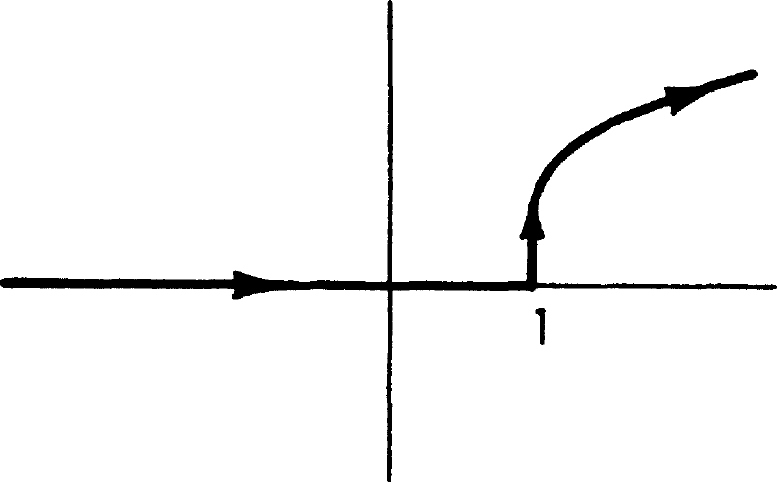
\includegraphics[scale=0.2]{FIGURAS/contorno}
	\caption{Deformación del contorno de integración lal plano complejo \cite{callan1977fate}.}
	\label{fig:contorno}
\end{figure}

\subsection{Trayectorias con múltiples bounces}

Como vimos en la sección \ref{sec:modo_zero}, el bounce no es único y existen otras trayectorias clásicas que también contribuyen a la amplitud de transición. De igual manera, debemos considerar la contribución de aquellas trayectorias que cuenten con un número arbitrario de bounces consecutivos lo suficientemente separados, aunque no sean soluciones exactas de la ecuación de movimiento \cite{weinberg2012classical}. 
%Además de los podemos tener un bounce seguido de otro, separados por un tiempo suficiente.  

Por comodidad, reescribamos $I_1$ 
%dado por la ecuación \eqref{eq:I_bounce} 
en función de $I_0$, 
\begin{equation} \label{eq:I1_I0}
	I_1 = iKTe^{-B/\hbar}I_0
\end{equation}
donde hemos definido 
 \begin{equation}
K \equiv \frac{1}{2} \left(\frac{B}{2\pi\hbar}\right)^{1/2} \left[ \frac{\textrm{det}' \left(-\dv[2]{}{\tau} + V''(x_B) \right)}{\det \left(-\dv[2]{}{\tau} + \omega^2 \right)}\right]^{-1/2}.
\end{equation}
De esta forma justificamos la elección de los subíndices puesto que estos señalan el número de bounces que contiene la trayectoria. 

Generalizando \eqref{eq:I1_I0}, tenemos que la contribución de una trayectoria que cuenta con $n$ bounces a la amplitud de transición $I_n$ está dada por
\begin{equation} \label{eq:I_n}
I_n = \frac{\left(iKTe^{-B/\hbar}\right)^n}{n!} I_0
\end{equation}
donde incluimos el factor de $n!$ debido a que los bounces son equivalentes y por lo tanto intercambiables entre sí. 

Con esto, solo queda sumar todas las contribuciones a la amplitud de transición
% de tal manera que esta está dada por
\begin{align}
	I &= \sum_{n = 0}^{\infty} I_n \\
	&= \sum_{n = 0}^{\infty} \frac{\left(iKTe^{-B/\hbar}\right)^n}{n!} I_0 \\
	&= I_0 \exp\qty(iKTe^{-B/\hbar})
\end{align}
y reemplazarlo en la ecuación \eqref{eq:Gamma}
\begin{align}
	\Gamma &= 2\Im\qty(\lim_{T \rightarrow \infty} \frac{ \ln \qty(I_0 \exp\qty(iKTe^{-B/\hbar}))}{T}) \\
	&= 2 \Im \qty(\lim_{T \rightarrow \infty} \qty( \frac{\ln I_0}{T} + iKe^{-B/\hbar})) \\
	%&= 2 \Im \qty(iKe^{-B/\hbar}) \\
	&= 2 Ke^{-B/\hbar}
\end{align}
de donde obtenemos finalmente que la tasa de decaimiento del falso vacío a primer orden en $\hbar$ está dado por
\begin{equation} \label{eq:gamma_final}
\Gamma = \left(\frac{B}{2\pi\hbar}\right)^{1/2}  \left[ \frac{\textrm{det}' \left(-\dv[2]{}{\tau} + V''(x_B) \right)}{\det \left(-\dv[2]{}{\tau} + \omega^2 \right)} \right]^{-1/2}e^{-B/\hbar}\left( 1 + \mathcal{O}(\hbar)\right).
\end{equation}
Notamos que \eqref{eq:gamma_final} es de la misma forma que \eqref{eq:gamma_WKB}, tal como esperábamos. Contamos ahora con una expresión analítica para la constante $A$ que, junto con la exponencial, representan el carácter no perturbativo del decaimiento del falso vacío \cite{weinberg2012classical}.  


